\section{绝对值}

\begin{definition}
    绝对值的代数意义：正数的绝对值是它本身，负数的绝对值是它的相反数， 0 的绝对值是 0 ，即：
    $$
        |a|= \begin{cases}a, & a>0 \\ 0, & a=0 \\ -a, & a<0\end{cases}
    $$
    绝对值的几何意义：一个数的绝对值，是数轴上表示它的点到原点的距离．
\end{definition}

\begin{theorem}[绝对值的性质]
    \begin{itemize}
        \item （1）$|a| \geqslant 0, \quad|a| \geqslant a, \quad|a| \geqslant-a$ ．
        \item （2）$|a|=|b| \Leftrightarrow a=b$ 或 $a=-b$ ．
              （ $\Leftrightarrow$ 表示左边可以推出右边，右边也可以推出左边）
        \item （3）$|a|^2=\left|a^2\right|=a^2,|a \cdot b|=|a| \cdot|b|,\left|\frac{a}{b}\right|=\frac{|a|}{|b|}(b \neq 0)$ ．
    \end{itemize}
\end{theorem}

\begin{warning}
    $|a|>|b| \Leftrightarrow a^2>b^2$ ．要注意很多错误的认识，如 $a>b \Leftrightarrow a^2>b^2$.
\end{warning}

\subsection{数轴上的距离}

\begin{theorem}[数轴上的距离]
    \begin{minipage}[c]{0.55\textwidth}
        在数轴上，如何求实数 $a, b$ 对应点 $A, B$ 之间的距离 $A B$ ？由于两个数的大小关系不明确，我们需要分类讨论：

        若 $a \geqslant b$ ，则 $A B=a-b$ ；若 $a<b$ ，则 $A B=b-a$ ．所以：
        $$
            A B= \begin{cases}a-b, & a \geqslant b \\ b-a, & a<b\end{cases}
        $$
        另一方面，对于 $|a-b|$ ，我们可以分情况讨论去掉绝对值符号：
        $$
            |a-b|= \begin{cases}a-b, & a \geqslant b \\ b-a, & a<b \end{cases}
        $$
        因此，在数轴上两点间的距离可以用绝对值表示：$AB = |a-b|$。
    \end{minipage}
    \hfill
    \begin{minipage}[c]{0.4\textwidth}
        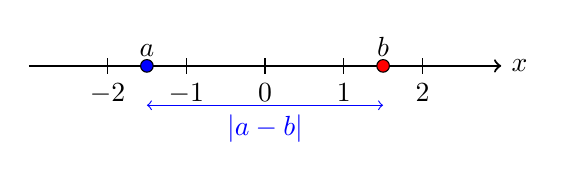
\begin{tikzpicture}
            % Draw the number line
            \draw[->, thick] (-3,0) -- (3,0) node[right] {$x$};

            % Draw tick marks
            \foreach \x in {-2,-1,0,1,2} {
                    \draw (\x,0.1) -- (\x,-0.1) node[below] {$\x$};
                }

            % Place points a and b
            \draw[fill=blue] (-1.5,0) circle (0.08) node[above] {$a$};
            \draw[fill=red] (1.5,0) circle (0.08) node[above] {$b$};

            % Draw the distance between a and b
            \draw[<->, blue] (-1.5,-0.5) -- (1.5,-0.5) node[midway,below] {$|a-b|$};
        \end{tikzpicture}
    \end{minipage}
\end{theorem}

\v{2em}

\begin{example}
    若数轴上的两点分别表示实数 $\boldsymbol{a}, \boldsymbol{b}$ ，那么这两点之间的距离表示 $|a-b|$.
    \begin{enumerate}
        \item 数轴上表示 -1 和 $x$ 的两点之间的距离是 \underline{\qquad}.
        \item 若数轴上一点表示 $\boldsymbol{x}$ ，则当代数式 $|x+1|+|x-1|$ 取最小值时，满足条件的整数 $\boldsymbol{x}$ 的值可以是 \underline{\qquad}.
    \end{enumerate}
\end{example}

\v{6em}

\begin{theorem}[数轴上的中点]
    $\frac{a+b}{2}$ 表示数轴上数 $a, b$ 对应的两点的中点所对应的数．
\end{theorem}

\begin{example}
    若在 $[0,3\pi]$ 上，方程 $\sin x = m (m > 0)$ 有四个解，分别为 $x_1, x_2, x_3, x_4$，请求 $x_1x_2x_3x_4$ 的最大值。
\end{example}

\v{8em}

\subsection{零点分段法}

在讨论含有绝对值的式子时，我们可以根据不同的零点来讨论：

\begin{example}
    化简：$|2 x+1|-|x-3|$ ．
\end{example}

\begin{solution}
    当 $x \geqslant 3$ 时，原式 $=(2 x+1)-(x-3)=x+4$；

    当 $-\frac{1}{2} \leqslant x<3$ 时，原式 $=(2 x+1)+(x-3)=3 x-2$；

    当 $x<-\frac{1}{2}$ 时，原式 $=-(2 x+1)+(x-3)=-x-4$ ．

    最后我们需要写成分段函数的形式：
    $$
        |2 x+1|-|x-3|= \begin{cases}
            x+4,   & x \geqslant 3              \\
            3 x-2, & -\frac{1}{2} \leqslant x<3 \\
            -x-4,  & x<-\frac{1}{2}
        \end{cases}
    $$
\end{solution}

\begin{example}
    解方程：$|x-2|+|x+1|=5$
\end{example}

\vspace{10em}

\subsection{讨论法解简单的绝对值不等式}

\begin{theorem}[简单的绝对值不等式]
    这里采用 $|a| < 5$ 作示例，应该变为：
    $$        -5 < a < 5$$
    也就是 $a$ 的取值范围是 $(-5, 5)$.

    如果里面是其他的整体，一样代换即可：
    $$ |2x+4| < 6$$
\end{theorem}

\begin{example}
    求 $|x^2+4x-4| < 5$ 的解集.
\end{example}

\v{8em}

\subsection{利用两边平方求解绝对值不等式}

\begin{theorem}[两边平方解绝对值不等式]
    平方保证了绝对值的非负性，绝对值之后得到的方程是一元二次方程。恰好符合绝对值不等式有两解的情况。
\end{theorem}

\begin{example}
    求下列不等式的解集：
    \begin{itemize}
        \item (1) $x(x+1) \leq 2 x+12$;
        \item (2) $|2 x-1|>x+3$;
    \end{itemize}
\end{example}

\v{4em}

\subsection{利用绝对值的解集确定参数的值}

\begin{example}
    已知函数 $f(x)=|x-a|-|2 x+1|, a \in \mathbf{R}$ ．
    \begin{itemize}
        \item 若 $f(x) \geq 0$ 的解集为 $\left[-3, \frac{1}{3}\right]$ ，求 $a$ 的值；
    \end{itemize}
\end{example}

\v{6em}
